

\Exercise[title={Integral delimitada entre funcions}]

%\begin{Exercise}[label=Ex7]
\Question
Sigui $S$ la regió delimitada  per les corbes $f_1(x)=x^2$, $f_2(x)=x$. Calculeu $\int \int_S (x+1)y dxdy$

%\end{Exercise}

\Answer

%  \begin{Answer}[ref=Ex7]

Comencem per dibuixar les dues funcions.

    \begin{center}
      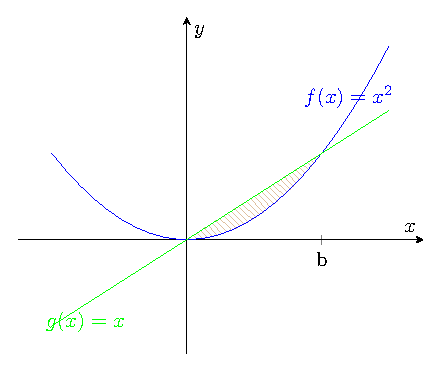
\includegraphics[width=0.5\textwidth]{areax2x.pdf}
    \end{center}

Es tallen en els punts $(0,0)$ i $(1,1)$, ja que
\[
  x^2=x \Rightarrow x^2-x=0 \Rightarrow x(x-1)=0
\]

La integració haurà de tenir en compte que la variable $x$ depèn de la $y$ i viceversa, per trobar el volum de l'objecte de la figura:

\begin{center}
  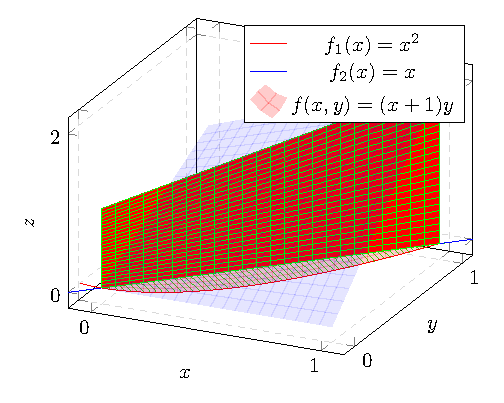
\includegraphics[width=0.5\textwidth]{volum3Dxx2xmes1y.pdf}
\end{center}

Per tant, una manera de solucionar el problema és:
\begin{eqnarray*}
V=\int \int_S (x+1)y dx dy &=& \int_{x=0}^{x=1} \left[ \int_{y=x^2}^{y=x} (x+1)y dy \right]dx \\
&=& \int_{x=0}^{x=1} \left[ \frac{(x+1)y^2}{2} \right]_{x^2}^{x} dx \\
&=& \frac{1}{2}\int_{x=0}^{x=1} \left[ (x+1)x^2 - (x+1)x^4 \right] dx\\
&=& \frac{1}{2}\int_{x=0}^{x=1} \left[ -x^5-x^4+x^3+x^2  \right] dx\\
&=& \frac{1}{2} \left[ -\frac{x^6}{6}-\frac{x^5}{5}+\frac{x^4}{4}+\frac{x^3}{3}\right]_{x=0}^{x=1}\\
&=& \frac{1}{2}\left[ \left(-\frac{1}{6}-\frac{1}{5}+\frac{1}{4}+\frac{1}{3}\right)-\left(0\right)\right]=\frac{13}{120}
\end{eqnarray*}


%\end{Answer}
